% Persoonlijk verslag van TinLab AA
% Mathematical Symbols:
% https://oeis.org/wiki/List_of_LaTeX_mathematical_symbols
\documentclass{article}% article report slides book letter beamer memoir minimal proc 
\usepackage{graphicx}
\usepackage{verbatim}% for multi line comments
\usepackage[dutch]{babel}
\usepackage{gensymb}% graden teken
\usepackage{multicol} %
\begin{document}
\sffamily
\begin{titlepage}
  \centering
    \vfill
    {\bfseries\Huge
      Verslag Tinlab Advanced Algorithms \\
        \vskip2cm
      }
      {\bfseries\Large
        J. I. Weverink\\
      }
      {
        \bfseries\normalsize
        \ldots\\
        \vskip1cm
        \today\\
    }    
    \vfill
    
\includegraphics[width=4cm]{pictures/logohr.png} % also works with logo.pdf
    \vfill
    \vfill
\end{titlepage}
\newpage
\tableofcontents

\newpage
\section{Inleiding}
Zie hier een referentie naar Royce~\cite{royce1987managing} en nog een naar Clarke~\cite{modelchecking}\ldots 

\section{Requirements}

\subsection{Requirements}
% Wat zijn requirements?
% behoefte of noodzaak
Requirements zijn beschrijvingen over hoe een product zou moeten functioneren. Zo verandert de betekenis van een requirement als de machine in een andere omgeving wordt geplaats. De requirements voor de verwaring van een ruimte bijvoorbeeld: Binnen moet het altijd warm zijn. In nederland kunnen we zeggen dat 25$^{\circ}$C als warm wordt aangezien. Terwijl op de noordpool dat op een lager punt zal zijn.

Anders gezegd zijn requirements geen harde eisen. Dit komt doordat de requirements zijn geformuleerd van het perspectief van de opdrachtgever. De opdrachtgever kan de requirtements geven zonder kennis te hebben van de machine die het moet gaan uitvoeren. De requirements die zijn opgesteld geven dan ook geen grenzen aan die overscheden kunnen worden.

% system requirements software requirements 
Onder requirements zijn er verschillende soorten requirements. Zo zijn system requirements opgesteld voor het hele systeem en bevatten subsystemen die die kunnen bestaan uit software en hardware. Hier moet uiteindelijk alles ervoor zorgen dat deze requirement wordt gehaald. Software requirement zijn niet bedoeld voor het hele systeem, maar behappen alleen de de software van het systeem. Software requirement zijn niet bedoeld voor het hele systeem, maar behappen alleen de software van het systeem. De software requirements kunnen gaan over over de functionele eisen, gebruikers eisen en zakelijke vereisten.
%software requirements: https://books.google.nl/books?hl=nl&lr=&id=nbpCAwAAQBAJ&oi=fnd&pg=PT32&dq=what+are+software+requirements&ots=9pK_H20xTk&sig=tEhuqR8M3pOWPPM4kDu4yOSfOys&redir_esc=y#v=onepage&q=what%20are%20software%20requirements&f=false
Requirements zijn onder te verdelen in verschillende delen: 
\begin{multicols}{2}
\begin{itemize}
\item Functional Requirement
\item Performance requirement
\item Usability requirement
\item User requirement
\item Interface requirement
\item Modes requirement
\item Adaptability requirement
\item Physical requirement
\item Design requirement
\item Enviromental requirement
\item Logistical requirement
\end{itemize}
\end{multicols}

%	https://www.sebokwiki.org/wiki/System_Requirements#Definition_and_Purpose_of_Requirements
% Hoe krijgt men requirements
% Wat voor requirements elication technieken zijn er zoal?
% 	functional, performance, constraint
% Wat is het verschil tussen functionelen en non--functionelen requirements?
Onder deze verschillende requirements zijn er nog twee soorten, functionele en niet-functionele requirements. 
Functionele requirements geven aan wat het systeem moet doen en kunnen. Niet-functionele requirements geven de eigenschappen aan van het systeem, zoals snelheid, veiligheid en bruikbaarheid. Met andere woorden functionele requirements geven informatie over het "wat". niet-functionele requirements geven informatie over het "hoe".

% wat is mode confusion?
\subsubsection{Mode confusion?}
De naam van het begrip zegt het eigenlijk allemaal. Bij mode confusion maakt de gebruiker een vergissing in de huidige of geactiveerde modus van het systeem. De gebruiker denk dat het systeem in modus A staat terwijl het werkelijk in modus B staat. 
%	mode van een apparaat bijv. auto in sport en eco modus

% Wat verstaat men onder automatiseringparadox
\subsubsection{Automatisering paradox}
Automatiseringsparadox. Wanneer een systeem is dat volledig geautomatiseerd moet worden is er altijd een wel een stap die dat nog niet is. Wanneer er een stap is geautomatiseerd moet er weer iets anders geautomatiseerd worden, om het hele systeem automatisch te krijgen.

\subsection{specificaties}
%system specifications	software specifications
Specificaties zijn eigenlijk niet heel veel anders dan requirements. ze beschrijven beide een systeem of een deelsysteem. Het grote verschil tussen de twee is de grenzen die ze opleggen. Bij requirements is er ruimte voor interpetatie, bij specificaties is die ruimte voor interpetatie er niet.

De specificaties geven geen ruimte voor interpetatie, omdat ze 'meetbare' informatie bevatten. In specificaties worden meetbare eenheden gebruikt, zoals 10 meter of 10$^{\circ}$C. Door dat de eisen een meetbare eenheid bevatten kan hiervan niet worden afgewezen. Deze specificaties zullen dan ook niet veranderen als het wordt gebruikt in een ander land, doordat de eenheden zijn gegeven.
\\

Stel we nemen het eerder genoemde requirement voorbeeld: "Binnen moet het altijd warm zijn." Als we dit vertalen naar een specificatie wordt het: "Binnen moet het altijd minimaal 20$^{\circ}$C zijn."

\clearpage
\subsection{Het vier variabelen model}
% Het 6 variable model
Sensoren Software Actuatoren Omgeving
\\
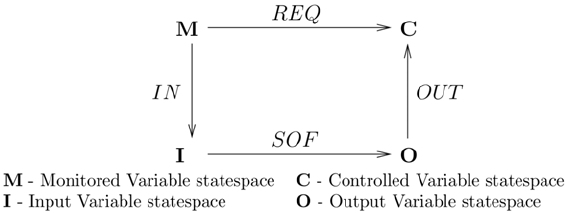
\includegraphics[width=10cm]{pictures/4_var_model.png}
\\
\cite{https://www.researchgate.net/figure/4-Variable-Model-of-Parnas-Madey_fig3_270733268}
% source https://www.researchgate.net/figure/4-Variable-Model-of-Parnas-Madey_fig3_270733268

\subsubsection{Monitored variabelen}
Wat gemeten wordt vanuit de omgeving:
\begin{itemize}
  \item Temperatuur
  \item Licht intensiteit
  \item Luchtvochtigheid
  \item Wat je allemaal met sensoren kunt meten
\end{itemize}

\subsubsection{Controlled variabelen}
Kunnen worden "bestuurd" door actuatoren:
\begin{itemize}
  \item Temperatuur
  \item Licht intensiteit
  \item Wat je allemaal kan beinvloeden
\end{itemize}

\subsubsection{Input variabelen}
De data, die staan voor de gemeten waardes vanuit de omgeving, die als input door de software worden gebruikt.

\subsubsection{Output variabelen}
De data die de software levert als output. Waar de actuatoren op moeten handelen.
% ===============================================================================
% ===============================================================================
% ===============================================================================
\subsection{Rampen}

\subsubsection{Ramp 1}
\begin{description}
\item[Beschrijving]
\item[Datum en plaats] 
\item[Oorzaak]
  %Beschrijf wat er mis ging in termen van het vier variabelen model/requirements/specificaties
\end{description}

\subsubsection{Ramp 2}
\begin{description}
\item[Beschrijving]
\item[Datum en plaats] 
\item[Oorzaak]
  %Beschrijf wat er mis ging in termen van het vier variabelen model/requirements/specificaties
\end{description}

\subsubsection{Ramp 3}
\begin{description}
\item[Beschrijving]
\item[Datum en plaats] 
\item[Oorzaak]
  %Beschrijf wat er mis ging in termen van het vier variabelen model/requirements/specificaties
\end{description}

\subsubsection{Ramp 4}
\subsubsection{Ramp 5}
\subsubsection{Ramp 6}

\section{Modellen}
Een goed model heeft een duidelijk object dat gemodelleerd moet worden, er is duidelijk \textbf{wat} er beschreven moet worden.
\\
Een goed model heeft een duidelijk doel.
-waarom modelleren we? (voor communicatie of verificatie, analyse, etc.)
\\
Een goed model is traceerbaar: elk onderdeel is te herleiden tot de onderdelen van het ëchte"systeem.
\\
Een goed model is waarheidsgetrouw: relevante onderdelebn van het model komen terug in de werkelijkheid.
\\
een goed model is eenvoudig, maar niet te eenvoudig
\\
Een goed model is uitbreidbaar en herbruikbaar: in de toekomst is het eenvoudig verder te werken met dit model en kunnen zelfs \textit{klassen} van vergelijkbare  systemen gemaakt worden
\\
Een goed model deelt geen jargon/semantiek met andere documenten en modellen.
\\\\
Richtlijnen (tegenstrijdig heden:
\\
Waarheidgetrouw vs simpelheid
duidelijheid vs. gedeeld jargon/semantiek
\subsection{De Kripke structuur}

\subsection{Soorten modellen}

\subsection{Tijd}

\subsection{Guards en invarianten}
Guards zijn voorwaarden waaraan moet worden voldaan voordat een status kan worden gemaakt.

\subsection{Deadlock}

\subsection{Zeno gedrag}

\section{Logica}

\subsection{Propositielogica}

\subsection{Predicatenlogica}

\subsection{Kwantoren}

\subsection{Dualiteiten}

\section{Computation tree logic}

\subsection{De computation tree}

\subsection{Operator: AG}
De betekenis van AG is makkelijk te onthouden A = Always, G = Globally. Dit houdt in dat het niet uit maakt waar je bent, je zal altijd van welke positie dan ook bij een gedefinieerd punt uitkomen.

\subsection{Operator: EG}
De betekenis van AG is makkelijk te onthouden E = Exists, G = Globally.

\subsection{Operator: AF}
De betekenis van AG is makkelijk te onthouden A = Always, F = Eventually.
\subsection{Operator: EF}

\subsection{Operator: AX}

\subsection{Operator: EX}

\subsection{Operator: p U q}

\subsection{Operator: p R q}

\subsection{Fairness}

\subsection{Liveness}

\newpage

\newpage
\bibliography{references}
\bibliographystyle{plain}
\end{document}


